\chapter{Investigations}
\label{chap:inv}
We perform preliminary investigations into assessing the dataset for later formulating the appropriate methodology that would best suit their innate properties.

\section{Attribution of Comments}
We seek an understanding of the strength of the association between comments and their authors. This would provide insight into user commenting behaviour, in particular whether a user has a unique vocabulary that distinguishes him from other users.

Authorship attribution aims at predicting the writer of a given a piece of text. In general a variety of stylometric and lexical features are used. Authorship attribution problems generally arise in forensic settings, and involve relatively long documents, and lists of possible authors limited to a few hundred candidate authors. Often, a sizable amount of example text is available for each candidate.In contrast, in our use case, the documents are short, the list of candidate authors is very large, and most are associated with little example text.                                          

\subsection{Literature}
Stamatatos provides an excellent summary of existing authorship attribution techniques \cite{stamatatos_survey_2009}. Most of the work discussed make use of both large documents and a smaller candidate author set. Stamatatos also points out that Support Vector Machines (SVM) perform extremely well as a distinguishing methodology in this particular scenario.

More recent work that looks into a smaller documents was done by Layton et al. \cite{layton_authorship_2010}, who look into authorship attribution for Twitter, where a micro-post (i.e., tweet) is restricted to 140 characters. Layton et al. opt for profile based feature representation of documents wherein all documents of a particular user are concatenated to form a super-document. They experiment with character $n$-grams with varying $n$ values and find that $4$-grams provide overall a good mean accuracy.

Work on large-scale attribution was carried out by Narayanan et al. \cite{narayanan_feasibility_2012}, who predict authors from a list of 100,000 candidate authors using a range of classifiers. Their dataset was comprised of blog posts, which are relatively longer than tweets or comments. They employed parts-of-speech tagging and a variety of lexical/character features for their purposes. A very interesting find in their work was that simple classifiers such as Naive Bayes and k-Nearest Neighbour performed better than SVM at the top ranks.

Our use case deals with shorter documents, namely comments, and a large candidate author set. We experiment with parts of methodologies adopted by Layton et al. \cite{layton_authorship_2010} and Narayanan et al. \cite{narayanan_feasibility_2012} as our problem is a combination of both. The upcoming sections discuss our methodology and the results of our experiments.

\subsection{k-NN Distance Based Attribution}
In our scenario, the training set is highly imbalanced, with a vast majority of authors having made very few comments and a handful of authors who made thousands of comments. For this reason, we adopt instance-based classification, wherein each document contributes on its own to the attribution and choose a simple 1-NN classifier.

For a given comment, we predict the nearest most resembling comment in the training set. It is to be noted that we do not make profile based predictions by grouping all comments of a single user together but rather each comment constitutes its own class. The overall framework is illustrated in Figure~\ref{fig:inv_1}.

\begin{figure}[!h]
\centering
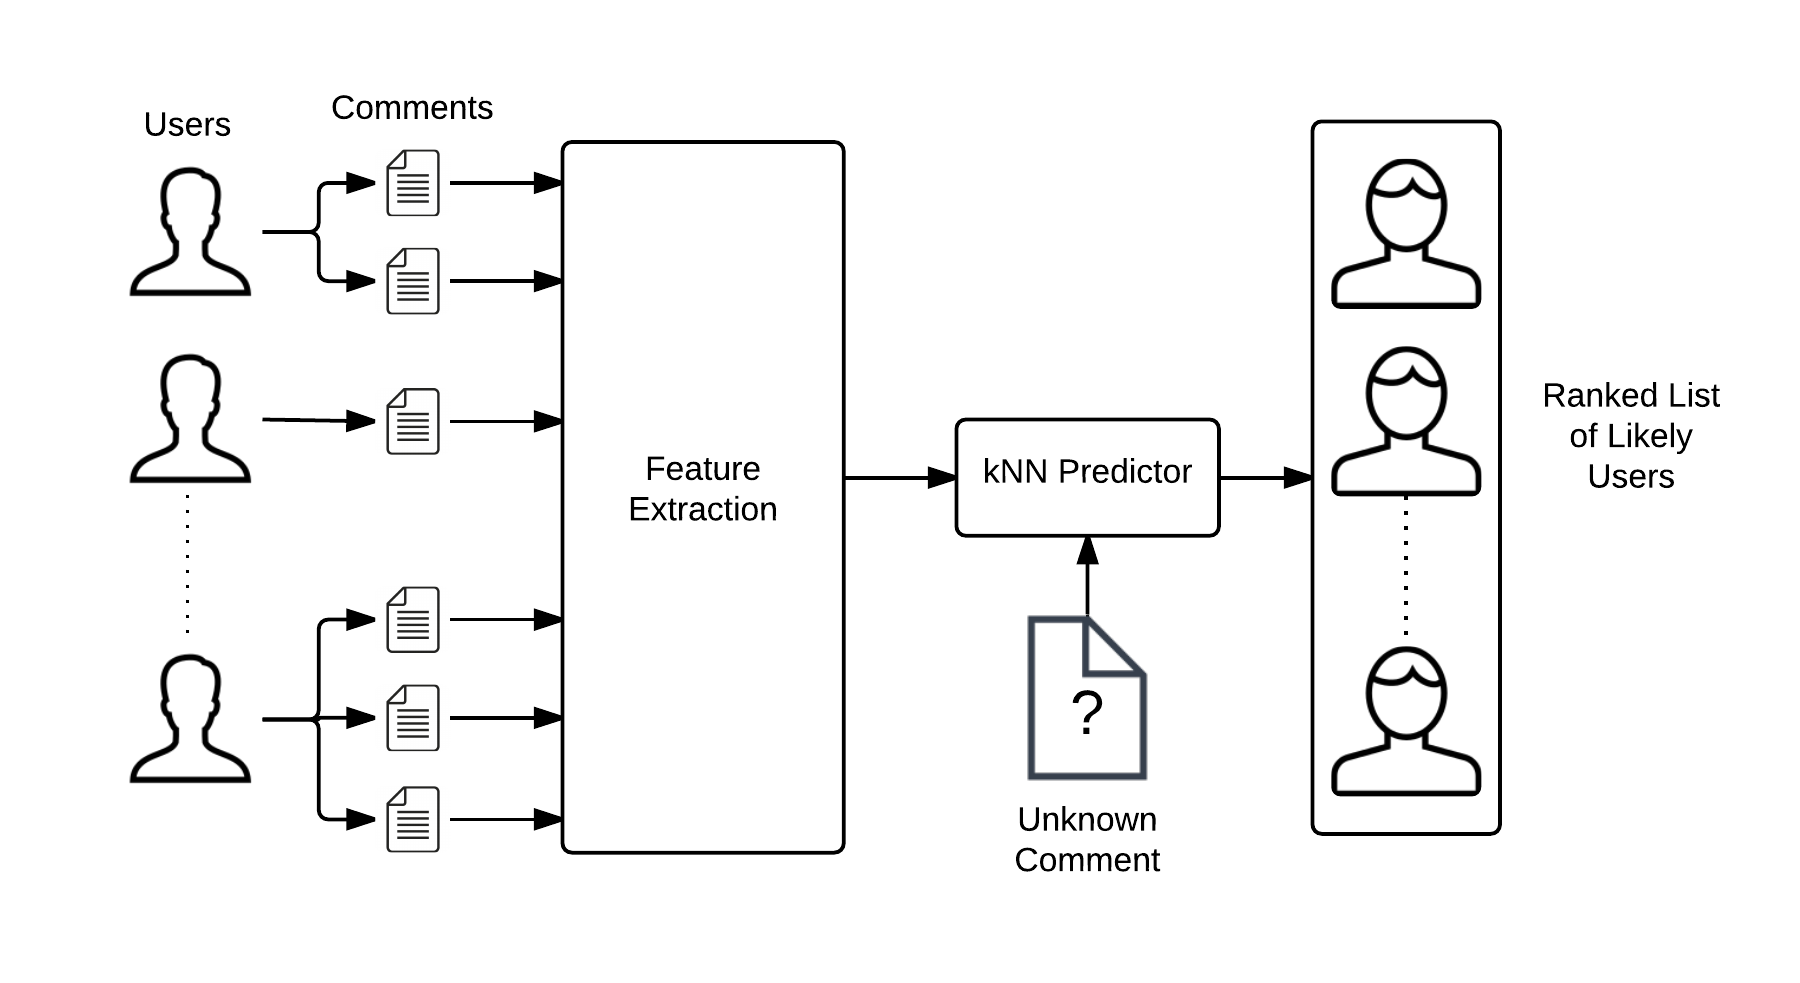
\includegraphics[width=1\textwidth]{c-inv_images/inv_1.png}
\caption{Authorship Attribution}
\label{fig:inv_1}
\end{figure}

The features we make use of are the character $n$-grams similar to that of Layton et al., since our use case also deals with similar informal text and shorter documents. We experiment with different values of $n$. We expect the value of $n$ to be important, since our data set is not homogeneously mono-lingual. We perform basic thresholding by selecting only those $n$-grams that occur more than five times in the entire dataset.

The character $n$-grams are converted into \textit{tf-idf} weight vectors, \textit{tf-idf} weights are essentially the product of the term frequency in a single document and the inverse document frequency. It aids in discerning the unique terms in a document thereby would directly expose user-specific features. Tf-idf is generally formulated as,

\begin{align*}
tfidf &= f_{t,d} * log\frac{N}{n_t}\\
\text{where, }& f_{t,d} \text{ - frequency of term $t$ in document $d$}\\
& N \text{ - total documents in corpus}\\
& n_t \text{ - number of documents with term $t$}
\end{align*}

Each vector represents a single comment and if a particular $n$-gram is not present then the corresponding \textit{tf-idf} entry is zero in that index. We experiment with two different distance functions as a means for finding their nearest neighbours. Namely, euclidean distance similar to what Narayanan et al. \cite{narayanan_feasibility_2012} used and cosine similarity. If $p_i$ and $q_i$ are two vectors then we formulate,

\begin{align*}
\text{Eucildean Distance} &= ||(q-p)||\\
\text{Cosine Similarity} &= \frac{p.q}{||p||*||q||}\\
\text{where, }||x|| &= \sqrt{x_1^2 + x_2^2 + x_3^ + ... + x_n^2} \text{ is the norm of the vector }x\\
\end{align*}

Euclidean distance directly measures the magnitude of the distance between the two vectors whereas cosine similarity measures the directional difference between the two vectors. 

\subsection{Attribution Experiments}
NU.nl comments are strictly moderated and the possibility of occurrence of spam is low, therefore we take the comments in their original form for $n$-gram tokenization without any form of filtering. The entire dataset encompasses over the last three months of 2014 as previously discussed in Chapter~\ref{chap:data}.

We partition the data temporally: the first 10 days of comments are taken as the training set and the next 3 days as the test set, we slide this 10-3 day split over the entire dataset, resulting in total of 79 samples of the data. Figure~\ref{fig:inv_2} better represents the sampling strategy.

\begin{figure}[!h]
\centering
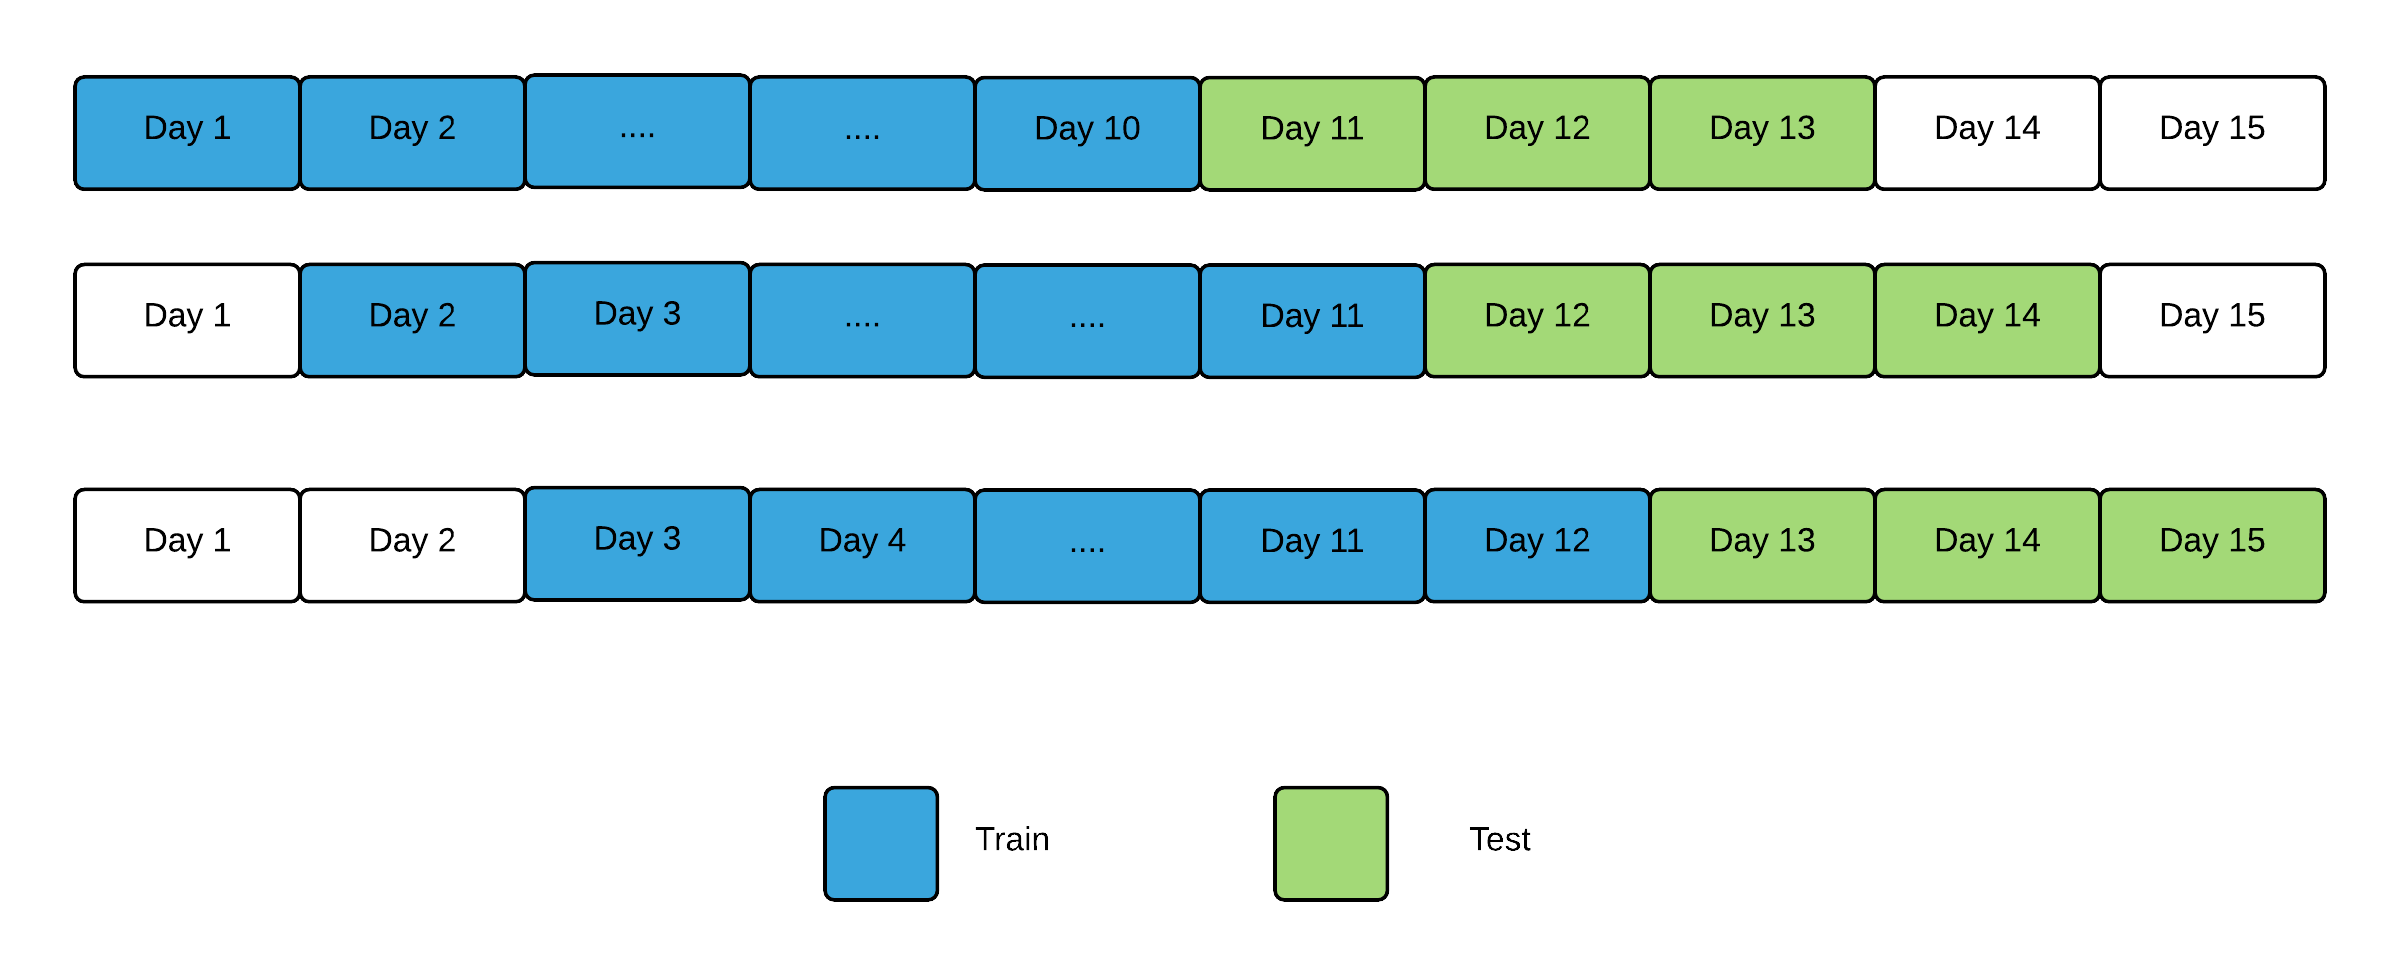
\includegraphics[width=1\textwidth]{c-inv_images/inv_2.png}
\caption{Sampling}
\label{fig:inv_2}
\end{figure}

This strategy was chosen since we are interested in predicting authorship based on historical data, and in any real world scenario, one can only predict future behaviour based on past instances and not the other way around. 

We also take into consideration only the candidate authors who had made at-least three comments, since we assume that it is not possible to make predictions with less data. Table~\ref{tab:split} shows the underlying split of the data averaged over all the samples.

\begin{table}[!h]
\centering
\begin{tabular}{|c|c|c|c|}
\hline
 \textbf{Train/Test} & \textbf{Average Users} & \textbf{Average Items} & \textbf{Average Comments} \\ \hline
 Train & 3930.55 & 1267.42 & 27275.09 \\ \hline
 Test & 3910.33 & 461.07 & 10356.82 \\ \hline
\end{tabular}
\caption{Data Split}
\label{tab:split}
\end{table}

The metric we use for evaluation is Mean Reciprocal Rank (MRR) which is %essentially 
the average of the reciprocal rank of the first hit in the list of candidates. We compute RR for those instances in which the author is found in the top 100 ranked results. For the rest of the cases, we assume that the author was ranked at infinity, and these cases contribute a RR of zero to the MRR. We also make use of $MAP@N$ which represents the mean average precision upto rank N.

As a sanity check, we calculated a trivial baseline that drew a comment from the training set at random. In essence, the baseline prioritizes users who have made more comments. The baseline had an $MRR < 0.001$ in both cases of NU and SC.

Table~\ref{tab:com_results} shows the results of classification averaged over all comments. 

\begin{table}[!h]
\centering
\begin{tabular}{|l|c|c|c|c|}
\hline
 \textbf{Distance Measure} & \textbf{n-gram} & \textbf{MRR} & \textbf{MAP@5} & \textbf{MAP@10}\\ \hline
 \multirow{3}{*}{Euclidean}& 2 & & & \\ \cline{2-5}
 & 3 & 0.0305 & 0.0141 & 0.0163 \\ \cline{2-5}
 & 4 & & & \\ \hline
 \multirow{3}{*}{Cosine} & 2 & &  & \\ \cline{2-5}
 & 3 & 0.0711 & 0.0357 & 0.0412 \\ \cline{2-5}
 & 4 & & & \\ \hline
\end{tabular}
\caption{Per-Comment Results}
\label{tab:com_results}
\end{table}

Clearly, the cosine similarity based prediction outperforms the euclidean distance based prediction. This may be due to the fact that cosine similarity outright ignores vectors which are entirely dissimilar whereas the euclidean distance measure does not. In the case of text, dissimilar vectors directly imply two pieces of text with entirely different words, this better suits our goal of trying to find similar comments.

But, it is open to question whether authorship attribution utilizing cosine similarity for all domains would outperform euclidean distance. Narayanan et al. \cite{narayanan_feasibility_2012} had used Euclidean distance for the special case of blogs which are much larger than comments and also a different set of features.

Considering the scale of results for our classification task wherein there were potentially around 4k different users to attribute to, we were able to make a prediction on average in the top 15 ranks. This implies that users of NU.nl more or less utilize the same words over time that makes them uniquely identifiable.

If one were to make use of conventional authorship features such as text compression, parts-of-speech, lexical features (frequency of punctuation, word length, sentence length), which capture subtle stylometric features rather than just the text, one might see an improvement over the base performance. But, use of such features is out of scope in this work. 

In the end we were still able to make decent predictions even without such advanced features and were able to assess that the average user of NU.nl utilizes the same vocabulary over time.

->TODO INSERT RANK GRAPHS

We also look into the stability of the predictions over different conditions so as to determine whether it is biased towards a particular nature of the dataset.

All plots are essentially histograms averaged with respect to the particular X-axis metric. Due to the wide variations that would potentially occur due to the wide range in the actual number of instances in each bin, we utilize Quantile Bounded Mean (QBM) as an approximation towards the trend of the plot.

To calculate the QBM approximation, we split our dataset that is binned with respect to the X-axis metric then split into 5\% quantiles. We then find the average over these quantiles resulting in a single data point for that quantile, connecting all such data points finally results in a smoothed approximation of the trend of the plot. We do not take into account the last quantile as it would contain potential outliers that are not characteristic of the entire dataset.

\begin{figure}[!h]
\centering
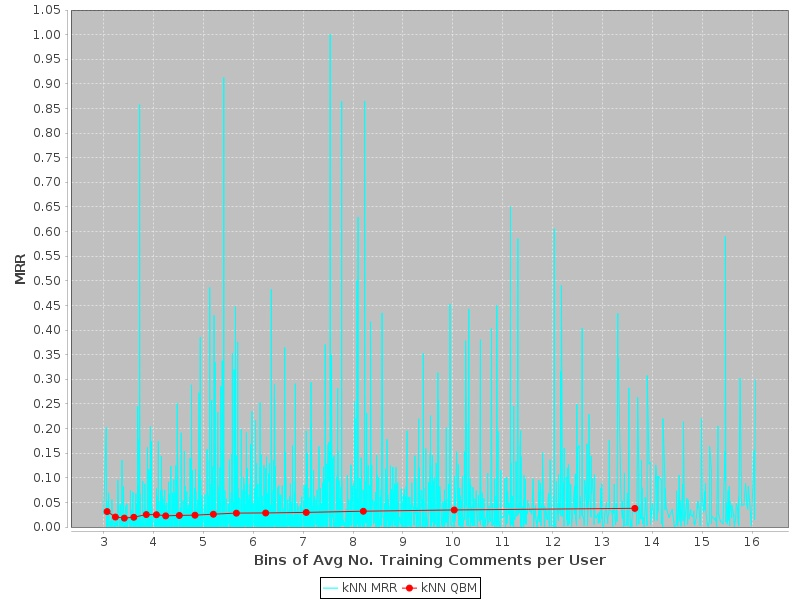
\includegraphics[width=0.75\textwidth]{c-inv_images/AuthorshipUserCountMRR.jpeg}
\caption{MRR Predictions vs No. Training Comments}
\label{fig:AuthorshipUserCountMRR}
\end{figure}

Figure~\ref{fig:AuthorshipUserCountMRR} is a plot of the MRR predictions versus the number of training comments that were utilized. As can be seen most of the instances occurred from 3-5 training comments, there is a slight fall between 3 and 4 but it picks up after 4 and generally stabilizes from there on. It is also to be noted that there are no drastic changes towards the end implying that more comments do not immediately imply better predictions. This also yields insight into the least number of comments required to make predictions - in this case 4 seems to be a good least threshold.

\begin{figure}[!h]
\centering
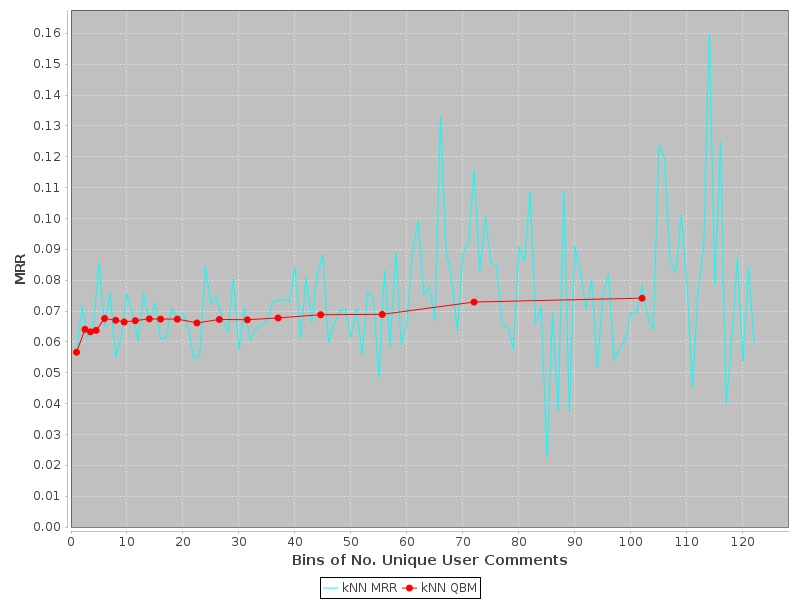
\includegraphics[width=0.75\textwidth]{c-inv_images/AuthorshipItemCountMRR.jpeg}
\caption{MRR Predictions vs No. Unique Users who Commented}
\label{fig:AuthorshipItemCountMRR}
\end{figure}

Figure~\ref{fig:AuthorshipItemCountMRR} is a plot of the MRR predictions versus the number of unique users who had commented on the item. This measure is essentially a surrogate of the popularity of the item - the more the unique users who commented the more popular the item is expected to be. There is a slight increase as the number of unique users increases - with a significant rise from 1 - 2 unique users and generally it stabilizes after 7 with slight increases towards the end. Yet again there are no drastic changes as observed previously.


\begin{figure}[!h]
\centering
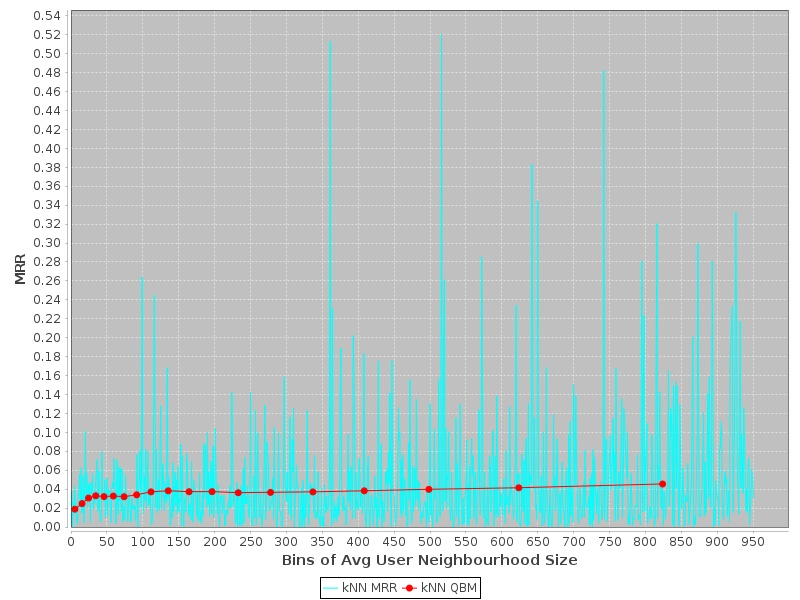
\includegraphics[width=0.75\textwidth]{c-inv_images/AuthorshipUserNeighMRR.jpeg}
\caption{MRR Predictions vs Neighbourhood Size of User}
\label{fig:AuthorshipUserNeighMRR}
\end{figure}

Figure~\ref{fig:AuthorshipUserNeighMRR} is a plot of the MRR predictions versus the user neighbourhood sizes. The user neighbourhood is simply computed by the sum of the unique users who co-commented along with the target user. The average neighbourhood size per user of the entire dataset was found to be 460.89 users. The MRR stabilizes after a neighbourhood size of ~30 implying that users who comment on items that are more often commented by other users are better attributed. But, similar to previous observations there are no drastic changes.

We further investigate the co-commenter behaviour by utilizing the target user's neighbourhood users' labels as the ground truth rather than only the target user's label. We utilize cosine distance for our predictions as we had previously observed that cosine distance performed better. Table~\ref{tab:co_com_results} shows the results of the co-commenter classification.

\begin{table}[!h]
\centering
\begin{tabular}{|l|c|c|c|c|}
\hline
 \textbf{(TODO ENTIRE DATASET) Predictor} & \textbf{n-gram} & \textbf{MRR} & \textbf{MAP@5} & \textbf{MAP@10}\\ \hline
 \multirow{3}{*}{k-NN Cosine} & 2 & &  & \\ \cline{2-5}
 & 3 & 0.3472 & &  \\ \cline{2-5}
 & 4 & & & \\ \hline
 \multirow{3}{*}{Random} & 2 & &  & \\ \cline{2-5}
 & 3 & 0.2150 & &  \\ \cline{2-5}
 & 4 & & & \\ \hline
\end{tabular}
\caption{Per-Comment Co-Commenter Results}
\label{tab:co_com_results}
\end{table}

A surprising observation was that random predictions perform close to that of our k-NN predictions. This is characteristic of the neighbourhood size - as we previously observed that the average neighbourhood size was 460.89 per user, considering this with the average number of users as seen in Table~\ref{tab:split}, in an ideal world scenario there would be ~9 clusters of users who comment on articles. Thereby it takes simply to find 1 of the 9 clusters to make a prediction.

As before, we investigate particular properties of the dataset and their influence on our predictions.

\begin{figure}[!h]
\centering
\begin{subfigure}[b]{0.475\textwidth}
    \centering
    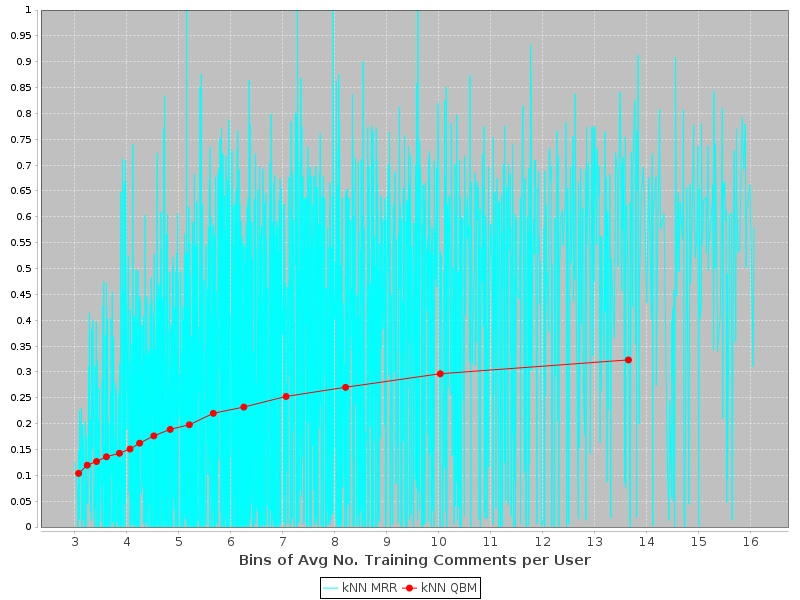
\includegraphics[width=\textwidth]{c-inv_images/co_AuthorshipUserCountMRR.jpeg}
    \caption{Cosine k-NN}
\end{subfigure}
\begin{subfigure}[b]{0.475\textwidth}
    \centering
    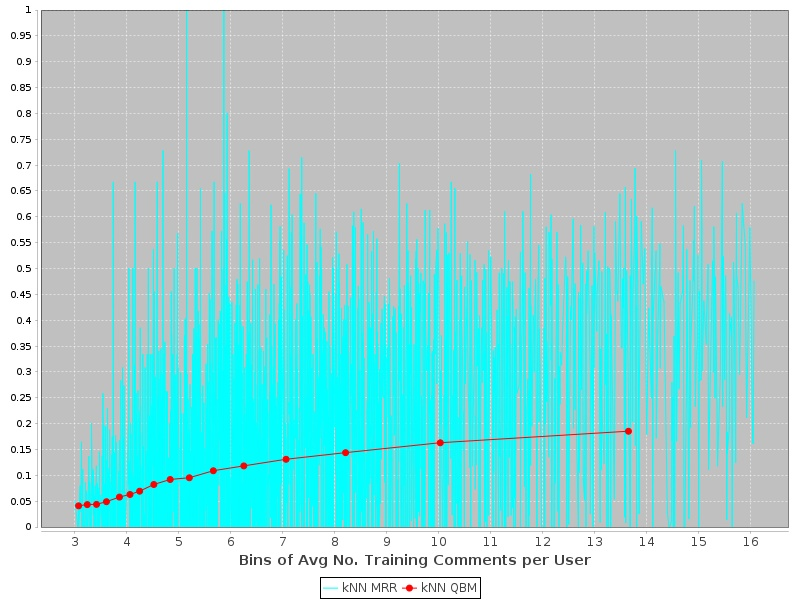
\includegraphics[width=\textwidth]{c-inv_images/randCo_AuthorshipUserCountMRR.jpeg}
    \caption{Random}
\end{subfigure}
\caption{Co-Commenter MRR Predictions vs No. Training Comments}
\label{fig:co_AuthorshipUserCountMRR}
\end{figure}

Figure~\ref{fig:co_AuthorshipUserCountMRR} is a plot of the co-commenter MRR predictions versus the number of training comments that were utilized. Both cosine k-NN and random predictions observe the same trend of gradual increase as the number of comments increases as increase in number of comments potentially increases the size of the ground truth labels under consideration.

\begin{figure}[!h]
\centering
\begin{subfigure}[b]{0.475\textwidth}
    \centering
    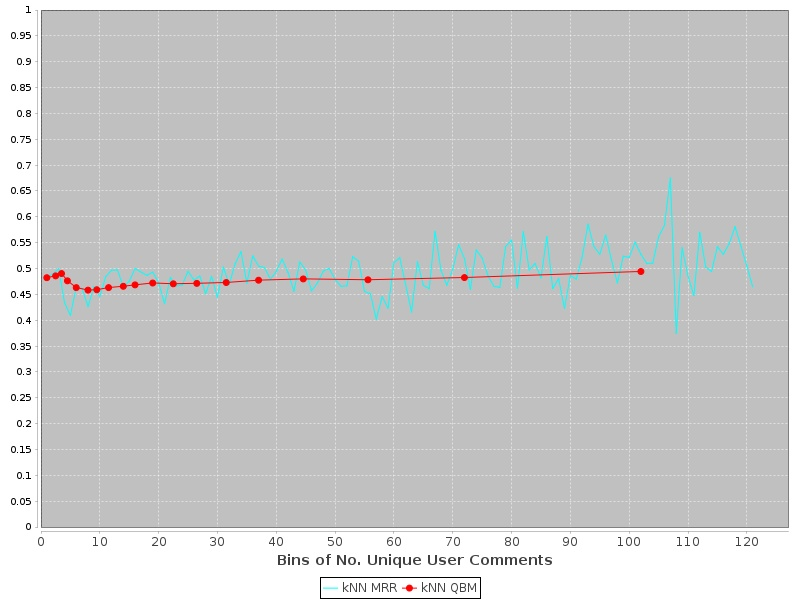
\includegraphics[width=\textwidth]{c-inv_images/co_AuthorshipItemCountMRR.jpeg}
    \caption{Cosine k-NN}
\end{subfigure}
\begin{subfigure}[b]{0.475\textwidth}
    \centering
    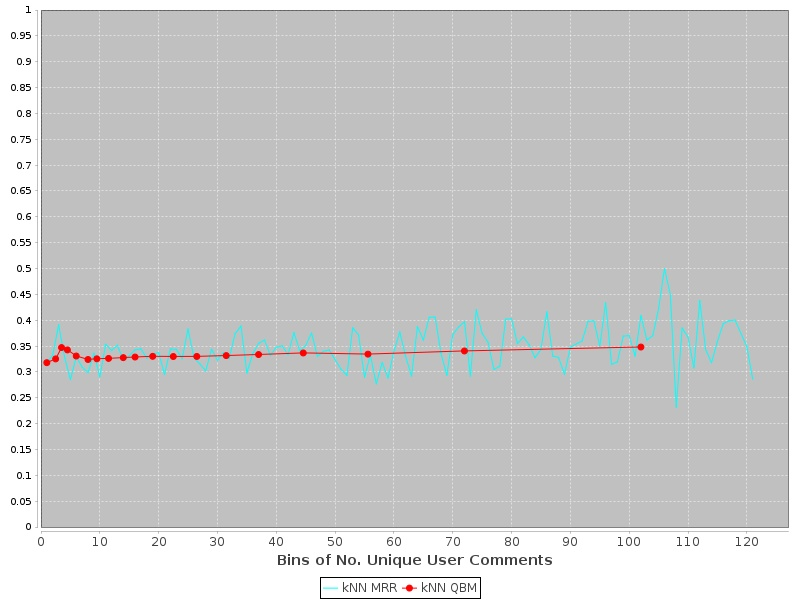
\includegraphics[width=\textwidth]{c-inv_images/randCo_AuthorshipItemCountMRR.jpeg}
    \caption{Random}
\end{subfigure}
\caption{Co-Commenter MRR Predictions vs No. Unique Users who Commented}
\label{fig:co_AuthorshipItemCountMRR}
\end{figure}

Figure~\ref{fig:co_AuthorshipItemCountMRR} is a plot of the MRR predictions versus the number of unique users who had commented on the item. Only earlier on, there is a slight rise and a subsequent fall whereas the rest is stabilized. This might be an indication that users with very large neighbourhood sizes comment on the least popular articles thereby causing a slight rise whereas the medium popular that ranges from ~7 are commented by the average user.

\begin{figure}[!h]
\centering
\begin{subfigure}[b]{0.475\textwidth}
    \centering
    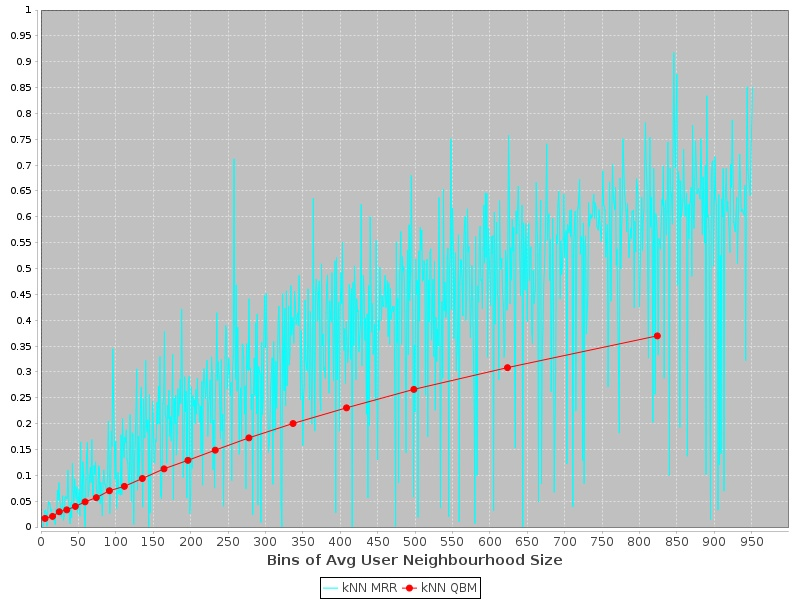
\includegraphics[width=\textwidth]{c-inv_images/co_AuthorshipUserNeighMRR.jpeg}
    \caption{Cosine k-NN}
\end{subfigure}
\begin{subfigure}[b]{0.475\textwidth}
    \centering
    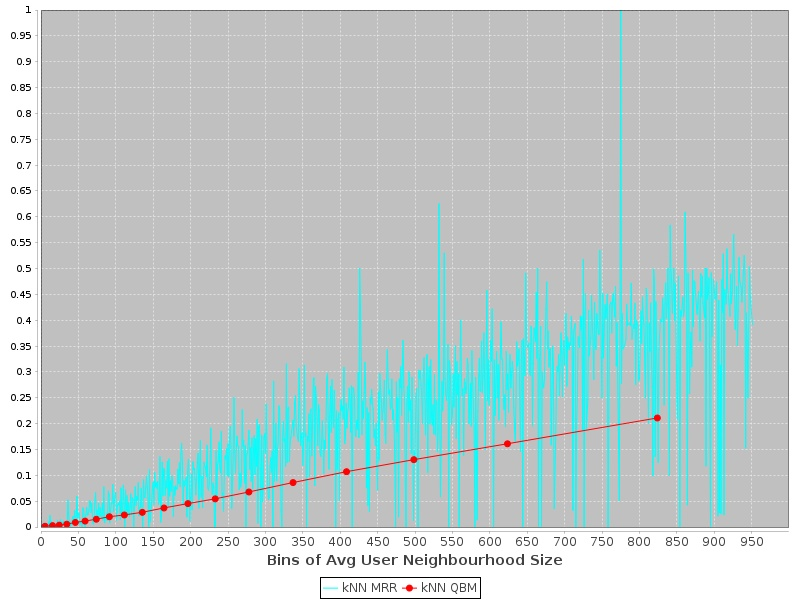
\includegraphics[width=\textwidth]{c-inv_images/randCo_AuthorshipUserNeighMRR.jpeg}
    \caption{Random}
\end{subfigure}
\caption{Co-Commenter MRR Predictions vs Neighbourhood Size of User}
\label{fig:co_AuthorshipUserNeighMRR}
\end{figure}

Figure~\ref{fig:AuthorshipUserNeighMRR} is a plot of the MRR predictions versus the user neighbourhood sizes. This without a doubt shows the anticipated that as the neighbourhood size increases, the number of ground truth labels increase and subsequently the MRR increases.

\subsection{Inferences}
In conclusion, we were able to make decent predictions for single label attribution even with simple features. For full fledged authorship attribution, one might employ the technique used here as a sampling strategy to narrow down a large number of authors to a candidate set that then later undergoes the entire process utilizing stylometric features for accurate prediction.

The co-commenter prediction shows the innate nature of the dataset wherein it is largely clustered into groups of users who consistently co-comment on the same set of items. Thereby potentially showing that collaborative filtering could be a good predictor in finding the items the target user would comment on. In addition, the accuracy of the single label attribution also encourages us to model the user by his unique vocabulary thereby use that as an indication of the user and not necessarily utilize the user's explicit label/id.